\documentclass[tikz,border=5pt]{standalone}
\usepackage[T1]{fontenc}
\usepackage{lmodern,amsmath,amssymb}
\usetikzlibrary{arrows.meta,calc,positioning,fit,backgrounds,shapes.geometric,matrix,decorations.pathreplacing,patterns}
\definecolor{ink}{gray}{0.08}
\definecolor{wash}{gray}{0.965}
\definecolor{soft}{gray}{0.45}
\tikzset{box/.style={draw=ink,line width=.65pt,fill=white,align=center,inner sep=4pt,outer sep=0pt,font=\small},flow/.style={draw=ink,line width=.65pt,-{Latex[length=1.8mm,width=1.3mm]},rounded corners=2pt},annotation/.style={font=\scriptsize,text=soft,align=center},groupbox/.style={draw=soft,dashed,line width=.45pt,fill=wash}}
\begin{document}
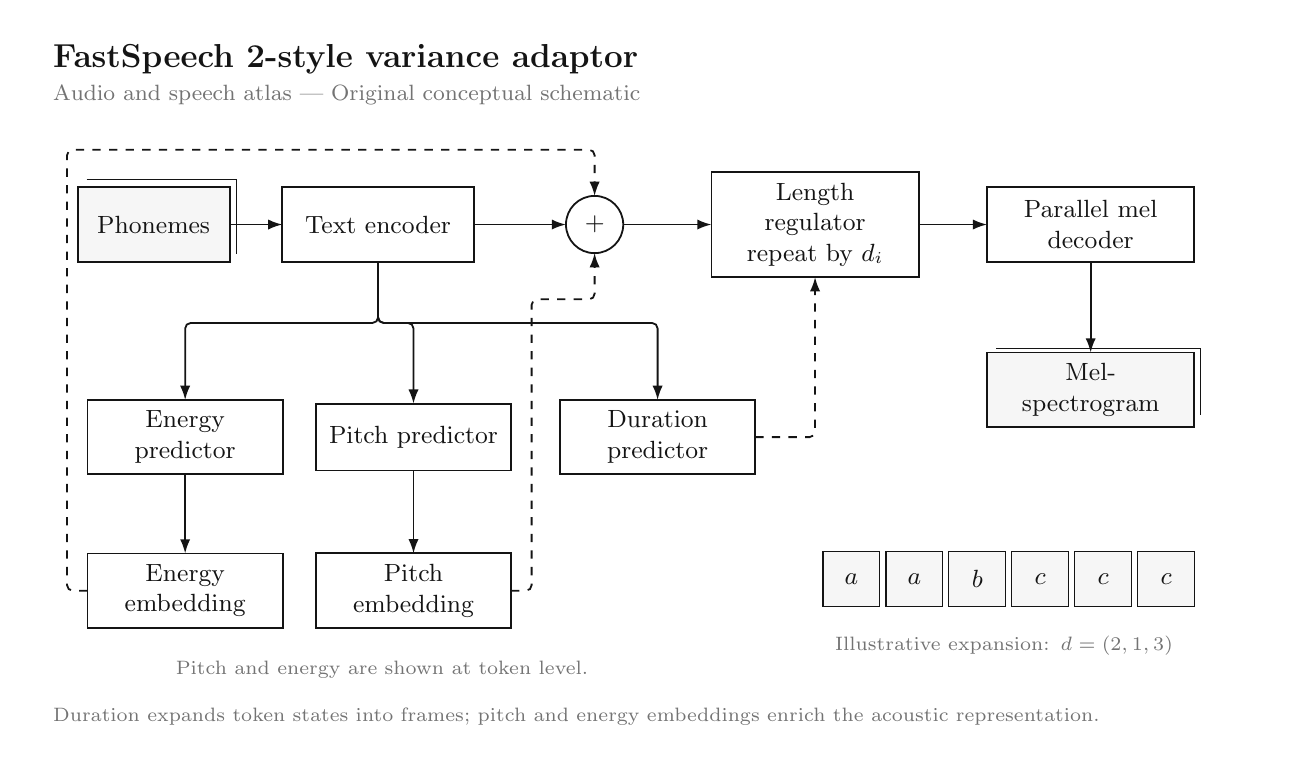
\begin{tikzpicture}[x=1cm,y=-1cm,font=\rmfamily,text=ink]

\path[use as bounding box] (0,0) rectangle (16,9);
\node[anchor=west,font=\large\bfseries] at (.2,.4) {FastSpeech 2-style variance adaptor};
\node[anchor=west,font=\footnotesize,text=soft] at (.2,.85) {Audio and speech atlas | Original conceptual schematic};
\begin{pgfonlayer}{background}
\end{pgfonlayer}
\node[box,fill=wash,minimum width=1.9cm,minimum height=0.95cm,text width=1.65cm] (text) at (1.6,2.5) {Phonemes};
\draw[ink,line width=.4pt] (0.7500000000000001,1.9249999999999998) -- (2.65,1.9249999999999998) -- (2.65,2.875);
\node[box,minimum width=2.4cm,minimum height=0.95cm,text width=2.15cm] (encoder) at (4.45,2.5) {Text encoder};
\node[box,circle,minimum width=0.5cm,minimum height=0.5cm,text width=0.25cm] (sum) at (7.2,2.5) {$+$};
\node[box,minimum width=2.6cm,minimum height=0.95cm,text width=2.35cm] (reg) at (10.0,2.5) {Length regulator\\repeat by $d_i$};
\node[box,minimum width=2.6cm,minimum height=0.95cm,text width=2.35cm] (decoder) at (13.5,2.5) {Parallel mel\\decoder};
\node[box,fill=wash,minimum width=2.6cm,minimum height=0.85cm,text width=2.35cm] (mel) at (13.5,4.6) {Mel-spectrogram};
\draw[ink,line width=.4pt] (12.299999999999999,4.075) -- (14.9,4.075) -- (14.9,4.925);
\node[box,minimum width=2.45cm,minimum height=0.85cm,text width=2.2cm] (energy) at (2.0,5.2) {Energy predictor};
\node[box,minimum width=2.45cm,minimum height=0.85cm,text width=2.2cm] (pitch) at (4.9,5.2) {Pitch predictor};
\node[box,minimum width=2.45cm,minimum height=0.85cm,text width=2.2cm] (duration) at (8.0,5.2) {Duration predictor};
\node[box,minimum width=2.45cm,minimum height=0.85cm,text width=2.2cm] (energyemb) at (2.0,7.15) {Energy\\embedding};
\node[box,minimum width=2.45cm,minimum height=0.85cm,text width=2.2cm] (pitchemb) at (4.9,7.15) {Pitch\\embedding};
\begin{pgfonlayer}{background}
\draw[flow] (text.east) -- (encoder.west);
\draw[flow] (encoder.east) -- (sum.west);
\draw[flow] (sum.east) -- (reg.west);
\draw[flow] (reg.east) -- (decoder.west);
\draw[flow] (decoder.south) -- (mel.north);
\draw[flow] (encoder.south) -- (4.45,3.75) -- (2.0,3.75) -- (energy.north);
\draw[flow] (encoder.south) -- (4.45,3.75) -- (4.9,3.75) -- (pitch.north);
\draw[flow] (encoder.south) -- (4.45,3.75) -- (8.0,3.75) -- (duration.north);
\draw[flow] (energy.south) -- (energyemb.north);
\draw[flow] (pitch.south) -- (pitchemb.north);
\draw[flow,dashed] (energyemb.west) -- (0.5,7.15) -- (0.5,1.55) -- (7.2,1.55) -- (sum.north);
\draw[flow,dashed] (pitchemb.east) -- (6.4,7.15) -- (6.4,3.45) -- (7.2,3.45) -- (sum.south);
\draw[flow,dashed] (duration.east) -- (10.0,5.2) -- (reg.south);
\end{pgfonlayer}
\draw[ink,fill=wash] (10.1,6.65) rectangle (10.82,7.35);
\node[align=center,anchor=center,font=\small,text=ink,text width=0.6cm] at (10.459999999999999,7.0) {\mbox{$a$}};
\draw[ink,fill=wash] (10.9,6.65) rectangle (11.620000000000001,7.35);
\node[align=center,anchor=center,font=\small,text=ink,text width=0.6cm] at (11.26,7.0) {\mbox{$a$}};
\draw[ink,fill=wash] (11.7,6.65) rectangle (12.42,7.35);
\node[align=center,anchor=center,font=\small,text=ink,text width=0.6cm] at (12.059999999999999,7.0) {\mbox{$b$}};
\draw[ink,fill=wash] (12.5,6.65) rectangle (13.22,7.35);
\node[align=center,anchor=center,font=\small,text=ink,text width=0.6cm] at (12.86,7.0) {\mbox{$c$}};
\draw[ink,fill=wash] (13.3,6.65) rectangle (14.020000000000001,7.35);
\node[align=center,anchor=center,font=\small,text=ink,text width=0.6cm] at (13.66,7.0) {\mbox{$c$}};
\draw[ink,fill=wash] (14.1,6.65) rectangle (14.82,7.35);
\node[align=center,anchor=center,font=\small,text=ink,text width=0.6cm] at (14.459999999999999,7.0) {\mbox{$c$}};
\node[align=center,anchor=center,font=\scriptsize,text=soft,text width=6cm] at (12.4,7.85) {Illustrative expansion: \mbox{$d=(2,1,3)$}};
\node[align=center,anchor=center,font=\scriptsize,text=soft,text width=8cm] at (4.5,8.15) {Pitch and energy are shown at token level.};
\node[anchor=west,align=left,font=\scriptsize,text=soft,text width=15.6cm] at (.2,8.75) {Duration expands token states into frames; pitch and energy embeddings enrich the acoustic representation.};
\end{tikzpicture}
\end{document}
